%============================================================
\chapter{Random Numbers and Deterministic Machines}\label{chap:randomNumbers}
\par{
The term {\em Entropy} is usually used  as the {\em measure of disorder 
and uncertainty of a system}.~\cite{Entrophy}. Claude E. Shannon defined it 
for information theory as the average of uncertainty (unpredictability) 
of an information source~\cite[p.~396]{AMathematicalTheoryOfCommunication}. 
The important properties of an information source with high entropy 
are~\cite[p.~150]{CryptographyAndNetworkSecurity}: 
\begin{description}
 \item [Uniform distribution:] Probability of each value should be the same, 
 no values should be generated with higher frequency of occurrence than others.
 \item [Independence:] No one value can be inferred from the others.
\end{description}
}

\par{
In this report the term {\em entropy} can also refer to a random value itself 
from an information source. 
}

\par{
\section{Pseudorandom Numbers}
When we pass any value to a {\em pseudorandom number generator} (PRNG), 
the PRNG will produce a long sequence of values, that seems to be random 
and statistical tests on these sequences (if the PRNG is strong enough) 
should not find any correlation between the produced values. However, 
the produced sequence is finite and thus after a time it become to repeat itself. 
This is because the PRNG is just an implementation of an algorithm, computing 
mathematical operations on the previously computed value (on the start 
of the PRNG, we need to fill it with a {\em seed} - a starting value) 
and after finite count of steps the algorithm gets to the point of its start.
}

\par{
A simple example of such PRNG, one of the most basic but the most widely 
used~\cite[p.~151]{CryptographyAndNetworkSecurity}, 
is the {\em linear congruential random number generator} (LCRNG) defined as 
\begin{equation}\label{eq:LCRNG}
  X_n = (aX_{n-1} + b) \mod{m}
\end{equation}
where $X_n$ is the $n$th number of the sequence ($X_{n-1}$ respectively 
the previous). $a$, $b$ and $m$ are constants and the selected values 
has big impact on quality of the output. $X_0$ is a seed. 
}

\par{
The LCRNGs are still useful because of their speed and easy implementation 
in various noncryptographic situations, when their disadvantages 
(most importantly their predictability~\cite[p.~152, 153]
{CryptographyAndNetworkSecurity}) 
are not important.~\cite[chapter~16.1]{AppliedCryptography}
}

\par{
Because with knowing the initial seed we can repeat all the pseudorandom 
sequence, it is important to have a secure, random seed if we want to use 
a PRNG in cryptography, except of having a {\em cryptographically secure 
pseudorandom number generator} (CSPRNG). In computers, the seed 
can be frequently extracted from hard-to-predict events like user interaction 
or network communication.
}

\par{
We can say a sequence generator is pseudorandom, if its output looks random, 
even under statistical tests.
}

\subsection{Cryptographically Secure PRNG}
\par{
Encryption algorithms can be sometimes used as the PRNG,
 for example DES or AES. These provide a very good 
 result~\cite[p.~153-156]{CryptographyAndNetworkSecurity}. 
 Using of an encryption algorithm is planned as a feature for the future version 
 of the library.
}

\par{
The important property of a PRNG, that can be considered as cryptographically 
secure, is {\em unpredictability}. That means that it is impossible under our 
computational knowledge to predict (forward or backward) any number, even if 
we know the used algorithm\footnote{This is the reason, why LCRNGs are not 
considered as CSPRNGs - if an attacker have just 3 following numbers 
of the basic LCRNG, $X_{i}$, $X_{i+1}$ and $X_{i+2}$, he can create 
an equation for each of them from the equation~\ref{eq:LCRNG} 
$X_n = (aX_{n-1} + b)$~mod~$m$. The three equations creates a system 
of equations with 3 unknowns $a$, $b$ and $m$, which is very easy to solve. 
After solving it, the attacker knows all the constants and then he can compute 
any preceding or following number in the sequence.} and/or the entropy 
source(s). The forward/backward security has to apply also for cases when 
the inner state of the RNG is disclosed, for example by reading it in memory.
}

\par{
The {\em forward security} grants us, that knowing of the current state 
of the generator, it is not possible to learn the previously generated values. 
The {\em backward security}, also known as {\em break-in recovery}  means, 
that even if an attacker knows the state of the generator in a specific time, 
it is not possible recover the state and thus predict future values.
}
\section{True Random Numbers}
\par{
To produce random values, {\em true random number generators} (TRNGs), 
are using physical events that are hard to be predicted. The TRNGs 
can measure absolute values, timing or occurrence of such events.
An examples of what can be used for generating true random numbers 
are radioactive decay, avalanche effects on reverse-biased electronic 
components and thermal, atmospheric and other sources of noise, 
and others~\cite[p.~6]{AnalysisOfEntropyLevels}.
}

\par{
However, real using of such devices is problematic. The sources of entropy are 
frequently somehow biased and cyclic, so it is necessary to have an online 
testing and filtering, which is usually significantly slowing the output speed. 
Also, the price can be a problem too\footnote{They usually cost from hundreds 
to thousands Euros. For a brief overlook, see a comparison 
on Wikipedia~\cite{HWRNGComparison}.}.
}

\section{Random Numbers in Linux}\label{sec:randomNumbers:linux}
\par{
The {\em Linux random number generator} (LRNG) is gathering its entropy 
from events that are very hard to predict: mouse movements, key-presses, 
interrupt sources of the system, jitter of access times to disks. 
These events are saved with a timestamp into an entropy 
pool~\cite{AnalysisOfLinuxRNG}.
}

\par{
LRNG is offering an API for its use. Except of C function 
{\tt get\_random\_bytes}, it also provides two device drivers, {\tt /dev/random} 
and {\tt /dev/urandom}. The difference between these two devices is in way, 
how they handle user requests, providing two different levels of security. 
The {\tt /dev/random} is producing more secure randomness and if there 
is not enough entropy in the entropy pool, then it can block the reader, 
until enough entropy is gathered. {\tt /dev/urandom} then never blocks its output
 and produce less secure values, but is faster\footnote{Just for illustration, 
 the speed of {\tt /dev/random} on my machine is about 300-400 KiB/s, 
 while {\tt /dev/urandom} is about 16 MiB/s}~\cite[chapter~1]{AnalysisOfLinuxRNG}. 
}

\par{
The LRNG is composed from three independent, asynchronous processes. 
Firstly, there is the collection of the entropy from all system. In the second 
process, the entropy is saved into the entropy pool and on last, when a random 
value is requested, the third process generates it using SHA-1 algorithm
\footnote{In all the process, the only one non-linear cryptographic function 
is SHA-1, that is used three times, along with some register shifting and pool 
mixing~\cite[section~2.6]{AnalysisOfLinuxRNG}.}~\cite[chapter~2]{AnalysisOfLinuxRNG}.
}

\begin{figure}[h!]
  \centering
 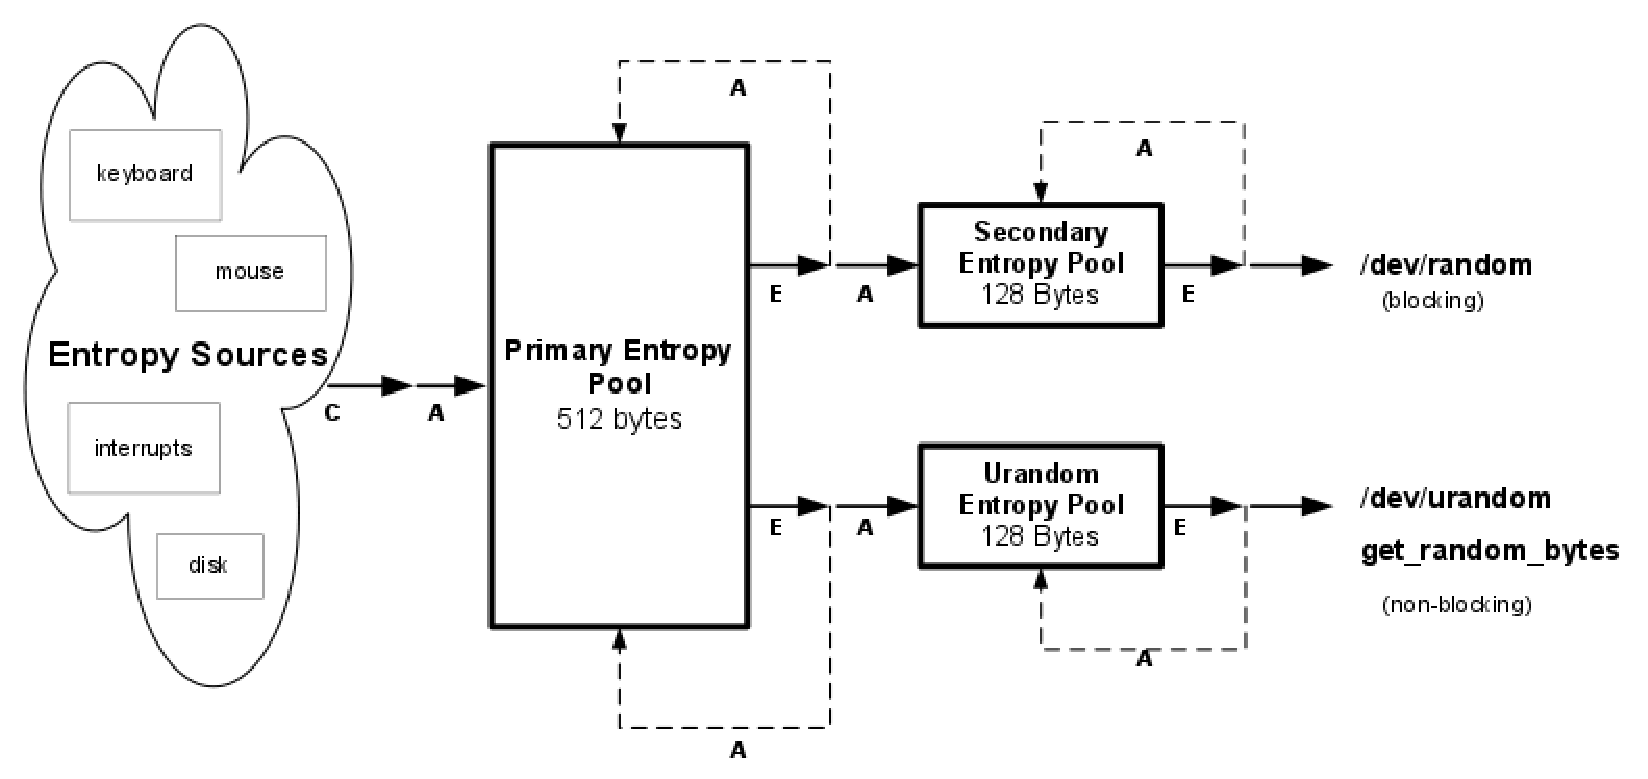
\includegraphics[width=16cm,keepaspectratio]{fig/LRNG} % Or .pdf
%\includegraphics[width=10cm,keepaspectratio]{fig/ISK-scheme}
\caption{Scheme of the LRNG. The entropy is collected (C) and added (A) 
to the primary pool. Entropy is extracted (E) from the secondary or urandom 
pool. Whenever entropy is extracted from a pool, some of it is also fed back 
into this pool (broken line). The secondary pool and the urandom pool draw 
entropy from the primary pool.~\cite{AnalysisOfLinuxRNG}}
\label{fig:LRNG}
\end{figure}

\par{
When a random value is generated, the process uses the relevant secondary 
or urandom pool as the seed and the level of entropy in the pool is lowered. 
When the level of entropy is too low, the pool is refreshed from the primary pool. 
In case of low entropy in all pools, the blocking {\tt /dev/random} waits until the 
system gathers more entropy, while {\tt /dev/urandom} just generates 
randomness from any entropy it has.
}
%-------------------------------------------------------------------------


\section{Summary}
\par{
As was noted, good true random number generators are hard to find, especially 
for an end-user usage. Although physical computers has some sources 
of entropy, with moving to virtualized systems the sources are 
disappearing~\cite{AnalysisOfEntropyLevels} and furthermore, with raising 
requirements of security, the importance of good random numbers is more 
important than before.
}

\par{
Also, as is showed in {\em Analysis of the Linux Random Number Generator}~\cite{AnalysisOfLinuxRNG}, 
even kernel generators can has security flaws and allow some form 
of forward or backward attack. 
}

\par{
For these reasons, it would be useful to have widely accessible and widespread
 fast and high quality TRNG or at least slower TRNG with CSPRNG. 
 That device should be available to all users, even within virtualized systems. 
 How RdRand can help with these points is shown in other chapters 
 of this thesis.
}